\documentclass{report}
% PACKAGES %
\usepackage[english]{} % Sets the language
\usepackage[margin=2cm]{geometry} % Sets the margin size
\usepackage{fancyhdr} % Allows creation of headers
\usepackage{xcolor} % Allows the use of color in text
\usepackage{float} % Allows figures and tables to be floats
\usepackage{appendix}
\usepackage{amsmath} % Enhanced math package prepared by the American Mathematical Society
	\DeclareMathOperator{\sech}{sech} % Include sech
\usepackage{amssymb} % AMS symbols package
\usepackage{mathrsfs}% More math symbols
\usepackage{breqn} % Allows splitting of long math lines
\usepackage{bm} % Allows you to use \bm{} to make any symbol bold
\usepackage{bbold} % Allows more bold characters
\usepackage{verbatim} % Allows you to include code snippets
\usepackage{setspace} % Allows you to change the spacing between lines at different points in the document
\usepackage{parskip} % Allows you alter the spacing between paragraphs
\usepackage{multicol} % Allows text division into multiple columns
\usepackage{units} % Allows fractions to be expressed diagonally instead of vertically
\usepackage{booktabs,multirow,multirow} % Gives extra table functionality
\usepackage{hyperref} % Allows hyperlinks in the document
\usepackage{rotating} % Allows tables to be rotated
\usepackage{graphicx} % Enhanced package for including graphics/figures
	% Set path to figure image files
	\graphicspath{{fig/}}
\usepackage{listings} % for including text files
	\lstset{basicstyle=\ttfamily\scriptsize,
        		  keywordstyle=\color{blue}\ttfamily,
        	  	  stringstyle=\color{red}\ttfamily,
          	  commentstyle=\color{gray}\ttfamily,
          	 }		

% Shortcuts for common numbers
\newcommand{\tab}{\-\hspace{1cm}}
\newcommand{\h}[1]{\section*{#1}}
\newcommand{\hh}[1]{\subsection*{#1}}
\newcommand{\hhh}[1]{\subsubsection*{#1}}

\newcommand{\p}{\partial}
\newcommand{\ppt}{\frac{\p}{\p t}}
\newcommand{\grad}{\vec{\nabla}}

\newcommand{\Xs}{\Sigma}
\newcommand{\xs}{\sigma}

\newcommand{\Oov}{\frac{1}{v}}

\newcommand{\pos}{\vec{r}}
\newcommand{\cur}{\vec{J}}
\newcommand{\Oh}{\hat{\Omega}}

\newcommand{\intfp}{\int_{4\pi}}
\newcommand{\intzi}{\int_0^{\infty}}


\newcommand{\rt}{(\pos,t)}
\newcommand{\rE}{(\pos,E)}
\newcommand{\rEprime}{(\pos,E')}
\newcommand{\rEO}{(\pos,E,\Oh)}
\newcommand{\rEt}{(\pos,E,t)}
\newcommand{\rEtprime}{(\pos,E',t)}
\newcommand{\rEOprime}{(\pos,E',\Oh')}
\newcommand{\rOt}{(\pos,\Oh,t)}
\newcommand{\rOtprime}{(\pos,\Oh',t)}
\newcommand{\rEOt}{(\pos,E,\Oh,t)}
\newcommand{\rEOtprime}{(\pos,E',\Oh',t)}
\newcommand{\EO}{(E,\Oh)}
\newcommand{\EOt}{(E,\Oh,t)}

\newcommand{\halflife}{T_{1/2}}

\newcommand{\uthree}{^{233}\text{U}}
\newcommand{\ufive}{^{235}\text{U}}
\newcommand{\ueight}{^{238}\text{U}}
\newcommand{\punine}{^{239}\text{Pu}}
\newcommand{\puone}{^{241}\text{Pu}}

\newcommand{\greens}{G(\pos,\pos')}
\newcommand{\oneDgreens}{G(x,x')}

% Create a header w/ Name & Date
\pagestyle{fancy}
\rhead{\textbf{Mitch Negus} \; NE250 - Nuclear Reactor Theory}

\begin{document}
\thispagestyle{empty}

{\bf {\large {Nuclear Engineering 250 -- Nuclear Reactor Theory \hfill Mitch Negus}}}


\h{Nuclear Reactions}

Two types


\hh{1. Spontaneous \textsl{(decay)}}

\begin{itemize}
    \item $\alpha$: $^A_ZX \rightarrow ^{A-4}_{Z-2}X + ^4_2\alpha$
    \item $\beta$: $^A_ZX \rightarrow ^A_{Z+1}X + \beta + \bar{\nu}$
    \item $\gamma$: $X^* \rightarrow X + \gamma$
\end{itemize}

\hhh{Decay Equations}
\begin{multicols}{2}
$ t \rightarrow N(t) $\\
$ t+dt \rightarrow N(t+dt) $\\
$dN(t) = N(t+dt) - N(t) $\\
$dN(t) = -\lambda N(t) dt$ where $\lambda$ is the decay constant.
\end{multicols}
... working through, with B.C. $N(t=0) = N_0$ ...
$$N(t) = N_0 e^{-\lambda t}$$

\hhh{Mean Lifetime:}
$\frac{dN(t)}{N_0} = \lambda e^{-\lambda t} dt = p_d(t)$ where $p_d(t) dt$ is the probability of decay in time $dt$
$$\bar{t} = \intzi t p(t) dt = \frac{1}{\lambda}$$

\hhh{Half-Life:}
$\halflife $is defined as the time s.t. $N(\halflife) = \frac{N_0}{2}$
$$\halflife = \frac{ln2}{\lambda}$$


\hh{2. Induced \textsl{(projectile/target)}}
\textsl{This will be the emphasis of NE 250}

\hhh{ Neutron-Nucleus}

\begin{itemize}
    \item elastic scattering
    \item inelastic scattering/compound nuclear reaction  
    $$n + ^A_ZX \rightarrow ^{A+1}_ZX^*$$
	(could result in production of a $\gamma$ or $\alpha$, emission of a $n$, or fission)
	
	\textbf{Capture is a subset of absorption!}\\
	Absorption: $(n,\alpha), (n,\gamma), (n,f)$\\
	Capture: $(n,\gamma)$
\end{itemize}
	
\textbf{Cross Sections ($\xs$)}\\
- A property of the isotope and reaction\\
- A function of the isotope temperature (vibrational motion) and neutron speed (linear motion)\\
- Tabulated in XSec libraries \textbf{(3 common formats)}
\begin{itemize}
    \item ENDF (USA)
    \item JEFF (Europe/NEA)
    \item JENDL (Japan)
\end{itemize}

\-\\
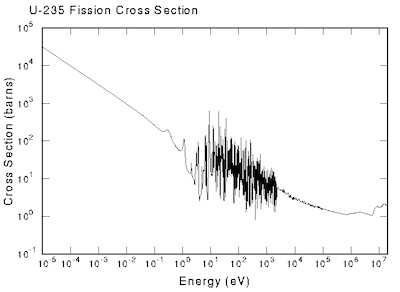
\includegraphics[width=10cm]{Lecture01_U235-Xsec}
\-\\

\begin{itemize}
    \item Resonances in X-Sec plots due to excited energy levels that can be reached; nuclei only all excitation to these levels, and so only neutrons with this energy amount will be absorbed
    \item Cross sections measured at 300K (room temp); calculated using
	$$ E = k_BT $$ where $k_B$ is Boltzmann's constant and $T=300 \text{ K} \Rightarrow E = 0.0253 \text{ eV}$
    \item Higher temperatures cause resonant peak widths to broaden (less time spent near center of vibrational trajectory) $\rightarrow$ \textbf{Doppler Broadening}
\end{itemize}
\-\\
\textbf{Units}\\
\tab $1 \text{ barn} = 10^{24} \text{ cm}^2$ \\ 
\tab $1 \text{ eV} = 1.602 \times 10^{-19} \text{ J}$


\hh{Fission}

Can be spontaneous or induced\\
$$ n + \ufive \rightarrow X + Y + \bar{\nu} n + E $$
$\bar{\nu}$ is the average number of neutrons produced in a given fission event.\\
$ E_f \approx 200 \text{ MeV} $ (this is much higher than chemical reactions which are on the order of eV!)

\hhh{Fissile Isotopes}
$ E_b > E_{\text{threshold}}$\\

These neutrons could (almost) be considered as "able to fission from 0 KE neutrons."

Includes $\ufive$, $\uthree$, $\punine$, $\puone$

\hhh{Fissionable Isotopes}

Fission requires collision with high $E$ neutrons.

For $\ufive$ this is empirically given by $$\chi(E) = 0.453e^{-1.036E}\sinh(\sqrt{2.29E})$$

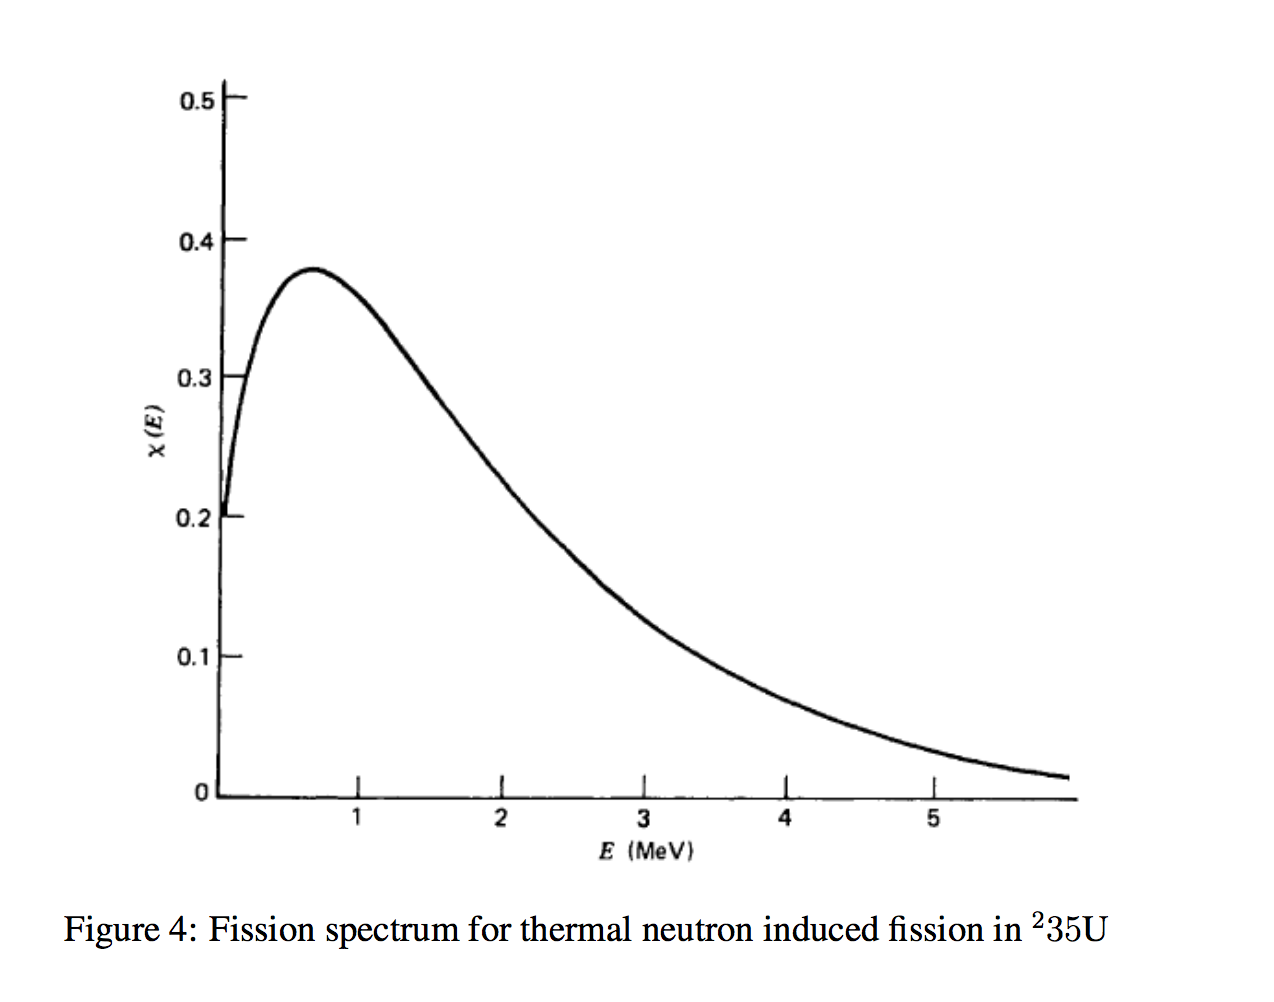
\includegraphics[width=10cm]{Lecture02_FissionEDist}


Also, note that $\bar{\nu}$ depends on the isotope. Below is a plot of $\bar{\nu}$ for $\punine$, $\uthree$ and $\ufive$:

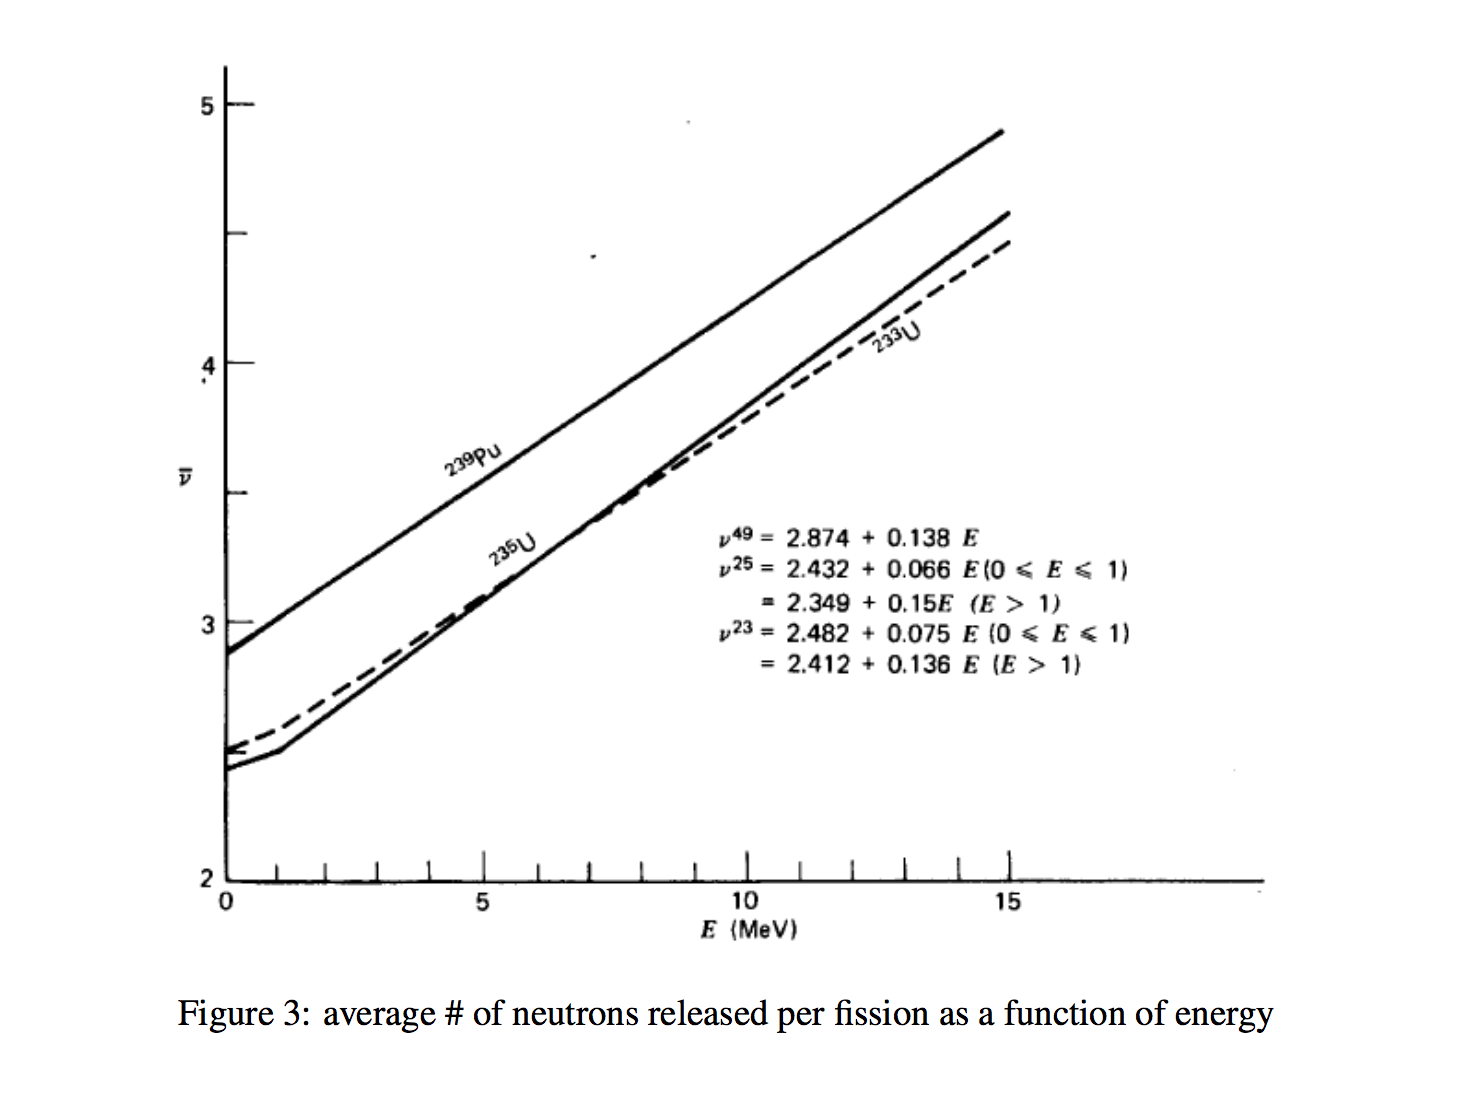
\includegraphics[width=10cm]{Lecture02_nubarUPu}

\hhh{Fertile Isotopes}

Isotopes which either undergo neutron capture (and subsequent decay) to become fissile isotopes.


\hh{Energy breakdown of fission outputs}

\begin{itemize}
    \item ~ 180 MeV in the KE of fission products
    \item ~ 5 MeV in the kinetic energy of neutrons
    \item ~ 7 MeV in prompt $\gamma$s
    \item ~ 8 MeV in $\beta^{-}$ decay of fission products
    \item ~ 7 MeV in delayed $\gamma$s
    \item ~ 12 MeV in neutrinos
\end{itemize}

The energy from all outputs can be captured except for neutrinos.



\h{Criticality}


\hh{Multiplication Factor, $k$}

$$ k = \frac{\text{\# neutrons generated}}{\text{\# neutrons lost}} $$

$\text{\# neutrons generated = neutrons fission}$\\ 
$\text{\# neutrons lost = \# neutrons absorbed + \# neutrons leaked}$

\begin{itemize}
    \item $k=1$: the reaction is critical; the chain reaction is controlled (reactor)  
    \item $k<1$: the reactor is subcritcal; boring  
    \item $k>1$: the reaction is supercritical; this is a bomb  
\end{itemize}


\hh{Derivation of the Neutron Transport Equation}

Solving for the multiplication factor requires that we know: 

\begin{enumerate}
    \item $n$: neutron density $[n/\text{cm}^3]$
    \item $N$: atom/nuclide density $[\text{nuclei}/\text{cm}^3]$
    \item $\xs$: microscopic cross section $[\text{cm}^2]$
\end{enumerate}

\textbf{Reaction rate:} $ \; R = n N \xs$\\
\textbf{Macroscopic cross section $[1/\text{cm}]$:} $ \; \Xs = N \xs $\\
\textbf{Angular neutron density $[\frac{n}{\text{cm}^3 \cdot \text{sr}}]$:} $\; n\rEOt$\\

$\vec{v} = v \,\Oh, \; |\Oh| = 1$ (describes a sphere, formed by $\theta$ and $\phi$)\\
$ dr^3 = dx \; dy \; dz$\\
$ dE$\\
$ d\Oh = \sin\theta \; d\theta \; d\phi$; $d\Oh$ is a scalar, about the original position defined by vector $\Oh$.\\

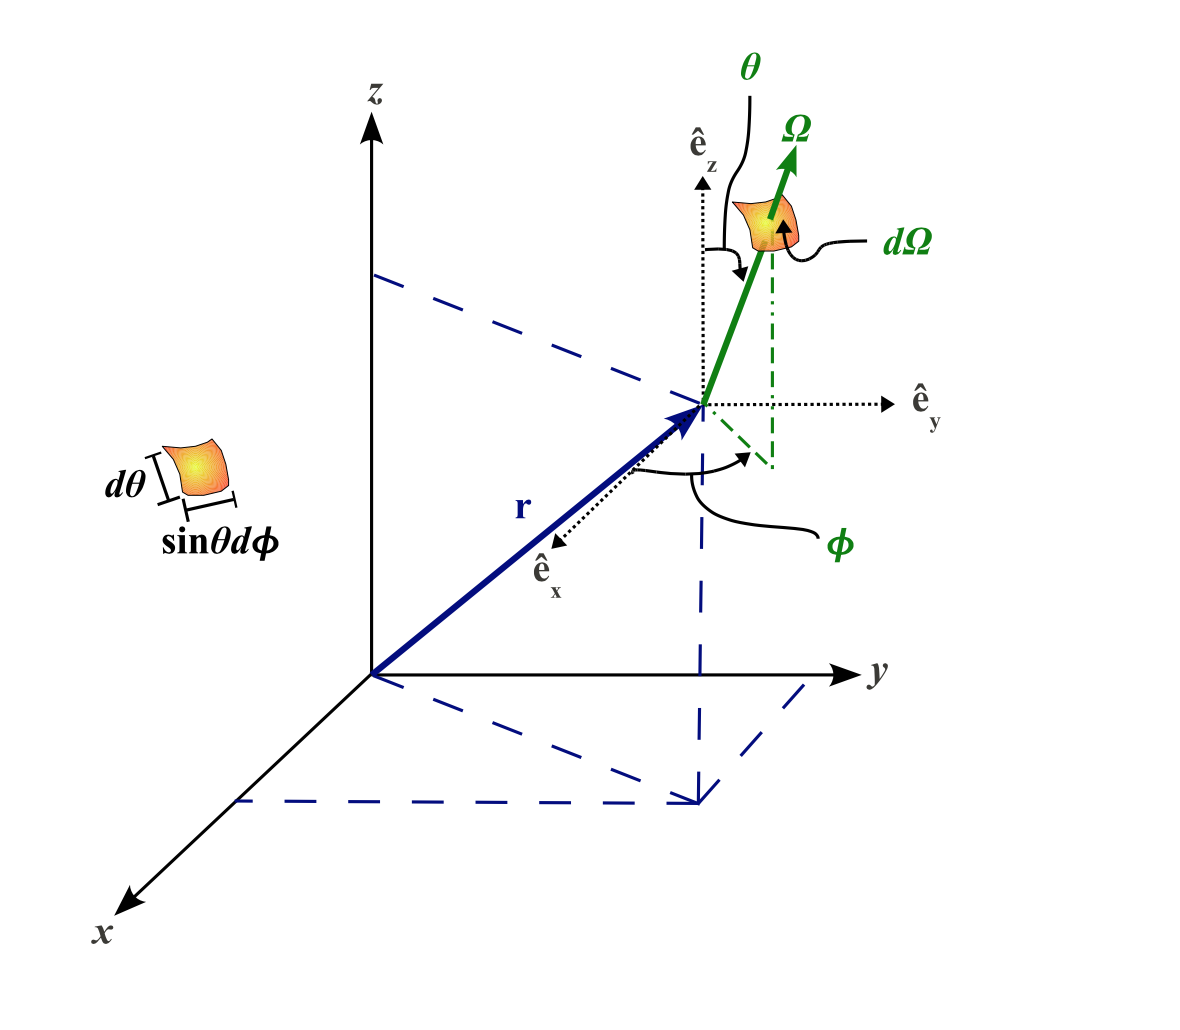
\includegraphics[width=10cm]{Lecture02_PhaseSpace.png}

Altogether, $ n\rEOt \; d^3r \; dE \; d\Oh$, gives the \# of neutrons in the small volume about $\pos$ with energy $E$, and moving in direction $d\Oh$ about $\Oh$ at time t.

\textbf{Angular neutron flux (scalar):} $\phi\rEOt = v \; n\rEOt$\\
\textbf{Angular neturon current (vector):} $\cur\rEOt = \Oh \; \phi\rEOt$\\

We can find the number of neutrons in a volume $V$ using
$$ \int_V{ n\rEOt \; d^3r }$$

Change with time is then 
$$ \ppt\left[\int_V{ n\rEOt \; d^3r }\right] dE \; d\Oh = \text{ \# neutrons gained - \# neutrons lost}$$

\# neutrons gained: source (fission), in-scattering ($E', \Oh' \rightarrow E, \Oh$)\\
\# neutrons lost: absorption, scattering ($E, \Oh \rightarrow E', \Oh'$)\\

We also add a streaming term, to quantify neutrons leaking out (and in) to the system.

The chance of a collision in the system is given by 
$$ \left[ \int_V{ \Xs_{\text{tot}}(\pos,E) v n\rEOt \; d^3r} \right] dE \; d\Oh $$

The chance of fission in system... 
\-\\
\-\\
\-\\
\-\\
$$\text{(See paper notes...)}$$



\h{The Transport Equation}

\begin{dmath*}
\Oov \frac{\p\psi}{\p t} + \Oh \cdot \nabla\psi + \Xs_t\psi = \intfp d\Oh'\intzi dE' \Xs_s(E',\Oh'\rightarrow E,\Oh)\psi(E',\Oh') + \frac{\chi(E)}{4\pi}\intzi dE'\nu(E')\Xs_f(E') \intfp d\Oh'\phi\rEOtprime + s\rEOt
\end{dmath*}
\-\\
\begin{multicols}{2}
\textbf{Initial condition:}
$\psi(\pos,E,\Oh,0) = \psi_0\rEO$

\textbf{Interface condition:}
angular flux must be continuous at all points
\end{multicols}

\hhh{Other conditions}
\tab \textbf{Fixed condition:} incoming flux is specified  
	$\psi(\pos_s,E,\Oh,t) = \psi_{\text{in}}\rEOt$\\
\tab\tab (Vacuum or black if $\psi_{\text{in}}\rEOt = 0$)\\
\tab \textbf{Reflective conditions:} mirror symmetry at some surface, $\psi(\Oh_{\text{in}},t) = \psi(\Oh_{\text{out}},t)$\\
\tab \textbf{Periodic conditions:} $\psi(\pos_s) = \psi(\pos_s + \vec{p})$\\
\tab \textbf{Finiteness conditions:} (can't have infinite flux)   
$0 \leq \psi\rEOt < \infty$\\
\tab \textbf{Source condition:} localized (pt.) sources introduce mathemetaical singularities\\
\tab\tab\tab\tab $S\rEOt = \lim_{\pos\rightarrow\vec{r_0}}\int dS \; \hat{e} \cdot \Oh$



\h{Approximations to the Transport Equation}


\hh{One-speed Transport Equation}

Assume all particles are the same speed: $\vec{v} = v_0 \cdot \Oh$

The equation becomes
$$ \Oov \frac{\p \psi\rOt}{\p t} + \Oh \nabla \psi \rOt + \Xs_t\psi \rOt = \intfp d\Oh' \Xs_s(\Oh'\rightarrow\Oh) \psi(\pos,\Oh',t) + \frac{\nu\Xs_f}{4\pi}\intfp d\Oh'\psi\rOtprime + S\rOt$$


\hh{One-dimensional}

$\pos = (x,y,z)$\\
$d\Oh = sin\theta \; d\theta \; d\varphi = d\mu \; d\varphi$, where $\mu = cos\theta$

$$ \Oov \frac{\p \psi(x,\Oh,t)}{\p t} + \Omega_x \frac{\p}{\p x} \psi (x,\Oh,t) + \Xs_t(x)\psi (x,\Oh,t) = \intfp d\Oh' \Xs_s(\Oh'\rightarrow\Oh) \psi(x,\Oh',t) + \frac{v\Xs_f}{4\pi}\intfp d\Oh' \psi(x,\Oh',t) + S(x,\Oh,t)$$



\h{The Diffusion Equation}

Usually the scalar flux is all that is needed to get a fairly accurate picture of our system. Reaction rates usually only depend on the neutron flux, not the direction of neutron motion.

\textbf{Assume} that the angular flux depends only weakly on direction.

\tab \textsl{Recall:}\\
\tab\tab\tab $\phi\rt = \intfp d\Oh \psi\rOt$\\
\tab\tab\tab $\cur\rt = \intfp d\Oh \; \Oh \;\psi\rOt$


\hh{The Neutron Continuity Equation}

\textbf{``The Zeroth Moment of the Transport Equation'':}\\
Integrate transport equation over all angles
\begin{dmath*}
\intfp d\Oh \left[\underbrace{\Oov\frac{\p \psi\rOt}{\p t}}_1 + \underbrace{\Oh \cdot \nabla \psi\rOt}_6 + \underbrace{\Xs_t \psi\rOt}_2 \right] = \intfp d\Oh \left[ \underbrace{\intfp d\Oh'\: \Xs_s(\Oh' \rightarrow \Oh) \psi\rOt}_5 + \underbrace{\frac{\nu \Xs_f}{4\pi} \intfp d\Oh'\: \psi\rOtprime}_3 + \underbrace{s\rOt}_4 \right]
\end{dmath*}

\begin{enumerate}
    \item \textbf{Time:} No approximations in time
$$ \Oov \ppt \intfp d\Oh \; \psi\rOt = \Oov \ppt \phi\rt $$

    \item \textbf{Absorption:} No approximations in absorption
$$\Xs_t \intfp d\Oh \; \psi\rOt = \Xs_t \; \phi\rt$$

    \item \textbf{Fission:} No approximations in fission
$$ \intfp d\Oh = \int_0^{\pi}\sin\theta \; d\theta \int_0^{2\pi} d\varphi = 4\pi$$
$$\intfp d\Oh \frac{\nu \Xs_f}{4\pi} \intfp d\Oh'\psi\rOtprime = \nu \Xs_f \phi\rt$$

    \item \textbf{Source:} No approximations in source 
$$\intfp d\Oh \; s\rOt \equiv S\rt$$

    \item \textbf{Scattering:} For scattering, interchange the order of integration
    $$ \intfp d\Oh \intfp d\Oh' \; \Xs_s(\Oh'\rightarrow \Oh) \; \psi\rOtprime = \intfp d\Oh' \intfp d\Oh \; \Xs_s(\Oh'\rightarrow\Oh) \; \psi\rOtprime$$

Now we assume that scattering is azimuthally symmetric (scattering depends only on cosine). The particle is as likely to scatter at angle $\theta$ in any direction off $ \Oh$.
    $$\intfp d\Oh \;\Xs_s(\Oh'\cdot\Oh) = 2\pi \int_{-1}^1 d\mu \; \Xs_s(\mu) = \Xs_s$$
Then, if we substitute this in above
    $$\Xs_s \intfp d\Oh' \; \psi\rOtprime =  \Xs_s \phi\rt$$

    \item \textbf{Streaming:} To adjust streaming, we first manipulate the order
$$ \intfp d\Oh \; \Oh \cdot \nabla \; \psi\rOt = \nabla \cdot \intfp d\Oh \; \Oh \; \psi\rOt = \nabla \cdot \cur\rt$$
\end{enumerate}

Put all the above integrations together to get the \textbf{neutron continuity equation (NCE)}. Notice that we have three equations (each $\pos$ has $x,y,z$ components) and 4 unknown quantities.

$$ \Oov \frac{\p \phi\rt}{\p t} + \nabla \cdot \cur\rt + \Xs_t \phi\rt = \Xs_s \phi\rt + \nu \Xs_f \phi\rt + S\rt $$


\hh{First angular moment}
Multiply the TE by $\Oh$ and integrate.  We will drop the fission term (technically we will assume it is part of the source), though the procedure is nearly the same when it is included.

Note:\\
\tab\tab $\intfp d\Oh \; \Oh = 0$\\
\tab\tab $\intfp d\Oh \; \Oh\Oh = \frac{4\pi}{3}\bar{\bar{I}}$, \tab $\bar{\bar{I}}$ is the identity tensor:  
	$$\intfp d\Oh \; \Oh_i\Oh_j = 
	\begin{cases}
	0, & i \neq j  \\
	\frac{4\pi}{3},&  i = j
	\end{cases}$$
\tab\tab $\intfp d\Oh \; \Oh\Oh\Oh = 0 $ 

When multiplied out, we have
$$ \intfp d\Oh \; \Oh\text{[TE]} $$
\begin{dmath*}
\underbrace{\intfp d\Oh \; \Oh \Oov \frac{\p \psi\rOt}{\p t}}_1 + \underbrace{\intfp d\Oh \; \Oh \Oh \nabla \psi \rOt}_5 + \underbrace{\intfp d\Oh \; \Oh \Xs_t\psi \rOt}_2 = \underbrace{\intfp d\Oh \; \Oh \intfp d\Oh' Xs_s(\Oh'\rightarrow\Oh) \psi(\pos,\Oh',t)}_4 + \underbrace{\intfp d\Oh \; \Oh \frac{\nu\Xs_f}{4\pi}\intfp d\Oh'\psi\rOtprime + \intfp d\Oh \; \Oh S\rOt}_3
\end{dmath*}

Like we did to derive the continuity equation, we can break down each term.
\begin{enumerate}
    \item \textbf{Time:}
    $$ \Oov \ppt \intfp d\Oh' \; \Oh\psi\rOt = \Oov \frac{\p\cur}{\p t} $$
    \item \textbf{Absorption:}
    $$ \Xs_t \intfp d\Oh \Oh\psi\rOt = \Xs_t \cur\rt $$
    \item \textbf{Source (fission now absent):}
    $$ \intfp d\Oh \; \Oh S\rOt \equiv S\rt $$
    \item \textbf{Scattering:} Expand scattering cross section in Legendre Polynomials (a sequence of orthogonal polynomials)
	$$P_n(x) = \frac{1}{2^n n!} \frac{d^n}{dx^n} \left[ (x^2 - 1)^n \right]$$
    Expand $\Xs_s(\Oh' \cdot \Oh)$ in Legendre polynomials
	$$ \Xs_s(\Oh' \cdot \Oh) = \sum_0^{\infty}{\frac{2\ell + 1}{4\pi}\Xs_{s\ell}P_{\ell}(\Oh')P_{\ell}(\Oh)} $$
	\begin{itemize}
	    \item $\ell = 0$ is isotropic\\ 
            \tab\tab\tab $P_0(\Oh) = 1 \quad\Rightarrow\quad \Xs_s(\Oh',\Oh) \approx \frac{1}{4\pi}\Xs_{s0}$
        \item $\ell = 1$ is linearly anisotropic\\  
            \tab\tab\tab $P_1(\Oh) = \Oh \quad\Rightarrow\quad \Xs_s(\Oh',\Oh) \approx \frac{1}{4\pi}(\Xs_{s0} + 3 \Oh' \cdot \Oh\Xs_{s1})$
            
            Assume scattering is at most linearly anisotropic (if its not, there's some "weird" stuff going on")
	\end{itemize}

	Substitute the linearly anistropic approximation into the expression for streaming. We note the prevously defined identities and defintion of neutron current:
	\begin{dmath*}
	\frac{1}{4\pi}\intfp d\Oh \Oh  \intfp d\Oh(\Xs_{s0} + 3 \Oh' \cdot \Oh\Xs_{s1}) \; \psi\rOt = \frac{1}{4\pi} \underbrace{\intfp d\Oh \; \Oh}_0 \intfp \Oh'\Xs_{s} \; \psi\rOtprime + \frac{1}{4\pi} \underbrace{\intfp d\Oh \; \Oh\Oh}_{4\pi/3\bar{\bar{I}}} \underbrace{\intfp d\Oh' \; \Oh' 3 \Xs_{s1} \; \psi\rOtprime}_{3\Xs_{s1}\cur\rt}
	\end{dmath*}
	
	Substituting those identities and simplifying, we get
	$$\left(\frac{1}{4\pi}\right) \left(\frac{4\pi}{3\bar{\bar{I}}}\right) \left(3\Xs_{s1}\cur\rt\right)= \Xs_{s1} \; J\rt$$


    \item \textbf{Streaming:}
	$$\intfp d\Oh \; \Oh \; \Oh \cdot \nabla \psi\rOt = \nabla \cdot \intfp d\Oh \; \Oh \;\Oh \; \psi\rOt $$

\end{enumerate}

Putting each of these 5 components back together the \textbf{current continuity equation (CCE)} is
$$\Oov \frac{\p \cur}{\p t} + \nabla \cdot \intfp d\Oh \;\Oh\Oh \; \psi\rOt + \Xs_t \cur\rt = \Xs_{s1}\cur\rt + S_1\rt$$

Now we have 2 moment equations (zeroth and first) so a total of 4 equations (neutron continuity and 3 tensor equations). There are now 10 unknowns: $\phi$ (1), $\cur$ (3), and the new tensor term (6). There is little point to continuing with this technique any longer.


\hh{Angular Flux Approximation}

Assume now that the flux is at most linearly anisotropic (for the current continuity equation we assumed that \textit{scattering} was linearly anisotropic).
$$ \psi(\Oh) \approx \frac{1}{4\pi}\left(\psi_0 + 3\Oh \cdot \vec{\psi_1}\right)$$

Substitute expansion into the streaming term of the current continuity equation.
$$\nabla \cdot \intfp d\Oh \;\Oh\Oh \; \psi\rOt = \nabla \cdot \intfp d\Oh \;\Oh\Oh \; \frac{1}{4\pi}\left(\psi_0 + 3\Oh \cdot \vec{\psi_1}\right)$$
$$ \nabla \cdot \frac{1}{4\pi} \int d\Oh \; \Oh\Oh \left(\psi_0 + 3 \Oh \vec{\psi_1}\right) = \nabla \cdot \frac{1}{4\pi} \left[ \intfp d\Oh \; \Oh\Oh \; \psi_0 + 3 \intfp d\Oh \; \Oh\Oh\Oh \; \vec{\psi}_1 \right] $$

Using the same identities as before, we have
$$ \nabla \cdot \frac{1}{4\pi} \int d\Oh \; \Oh\Oh \left(\psi_0 + 3 \Oh \vec{\psi_1}\right) = \nabla \cdot \frac{1}{4\pi} \frac{4\pi}{3}\bar{\bar{I}} \; \phi\rt $$
(Note, that this assumes $\psi_0 = \phi \leftarrow$ figure out where this comes from)
and
$$ \nabla \cdot \frac{1}{4\pi} \int d\Oh \; \Oh\Oh \left(\psi_0 + 3 \Oh \vec{\psi_1}\right) = \frac{1}{3} \nabla \phi\rt $$

Now the current continuity equation is 
$$\Oov \frac{\p \cur}{\p t} + \frac{1}{3} \nabla \phi\rt + \Xs_t \cur\rt = \Xs_{s1}\cur\rt + S_1\rt$$

Define absorption and transport cross sections:\\
$\Xs_a \equiv \Xs_t - \Xs_{s0}$\\
$\Xs_{tr} \equiv \Xs_t - \Xs_{s1}$\\

Using these cross sections we can reform both the neutron and current continuity equations.

\textbf{NCE:}
$$ \Oov \frac{\p \phi\rt}{\p t} + \nabla \cdot \cur\rt + \Xs_a \phi\rt = S\rt $$
\textbf{CCE:}
$$\Oov \frac{\p \cur}{\p t} + \frac{1}{3} \nabla \phi\rt + \Xs_{tr} \cur\rt = S_1\rt$$


\textbf{Fick's Law}\\

With the following conditions
\begin{itemize}
    \item Steady state $(\ppt(X) = 0)$
    \item Isotropic source ($S_1 = 0$)
\end{itemize}

The current continuity equation becomes
$$\frac{1}{3} \nabla \phi(\pos) + \Xs_{tr} \cur(\pos) = 0$$
which we can solve for $\cur$:
$$\cur(\pos) = -\frac{1}{3\Xs_{tr}} \nabla \phi(\pos).$$
If we let $D = \frac{1}{3\Xs_{tr}} = \frac{1}{3(\Xs_t-\Xs_{s1})}$ be the diffusion coefficient, then this simplifies further to
$$\cur(\pos) = -D \nabla \phi(\pos)$$

------------------------------------------------------------------\\
Recall:\\
$\Xs_{s1} = \int d\Oh \; \Oh \Xs_{s}$\\
Include azimuthally symmetric assumptions and $\Xs_{s1} = \bar{\mu}_0 \Xs_s$, where $\bar{\mu}_0$ = average scattering cosine = $\frac{2}{3A}$, where $A$ is the atomic mass number.

Then $\Xs_{tr} = \Xs_t - \bar{\mu}_0 \Xs_s$.\\
------------------------------------------------------------------\\

From this implementation of Fick's law, we can write the diffusion equation as only a function of $\phi$:

$$\Oov \ppt \phi\rt - \nabla \cdot D \nabla \phi\rt + \Xs_a \phi\rt = \nu\Xs_f \phi\rt + S\rt$$

Due to our assumptions, however, the diffusion equation is not valid at 
\begin{enumerate}
    \item Boundaries/interfaces
    \item Sources
    \item Strong absorbers
    \item Voids
\end{enumerate}

The angular flux expansion can then be written as 
$$\psi\rOt \approx \frac{1}{4\pi}\left( \phi\rt - \frac{1}{\Xs_{tr}} \nabla \phi\rt \right)$$

At equilibrium, $\cur = 0$ (net migration is opposed to gradient, hence negative into Fick's Law)

\textbf{Mean Free Path:} the median distance from the last collision\\
$\lambda_t = \frac{1}{\Xs_t}$ or $\lambda_{tr} = \frac{1}{\Xs_{tr}}$

If scattering is 
\begin{itemize}
    \item isotropic $\rightarrow \bar{\mu}_0 = 0, \lambda_t = \lambda_{tr}$
    \item forward peaked $\rightarrow \bar{\mu}_0 > 0, \lambda_t > \lambda_{tr}$
\end{itemize}
\-\\

\begin{multicols}{2}
\hhh{Initial Conditions:} 
$\phi(\pos,0) = \phi(\pos) \; \forall \pos \in V$

Basic requirements:\\
- real and nongegative ($\phi \geq 0$)\\
- bounded ($\phi > \infty$) \\

\hhh{Interface conditions:} 
-Zeroth and first moments must be continuous\\
\tab$\phi_1\rt = \phi_2\rt$\\
\tab$\cur_1\rt = \cur_2\rt$\\

\columnbreak
\hhh{Vacuum BCs:}
%$\psi\rsOt = \Oh \hat{e}_s < 0$\\
In the DE use partial current\\
\tab $J_{-}\rt = \int_{2\pi^{-}} d\Oh \Oh \cdot \hat{e}_s \psi\rOt = 0$\\
\tab $J_{+}\rt = \int_{2\pi^{+}} d\Oh \Oh \cdot \hat{e}_s \psi\rOt = 0$\\

$J_{\mp} = \int_{2\pi^{-}} d\Oh \Oh \hat{e}_s \left( \frac{1}{4\pi} \left( \phi \pm \frac{1}{\Xs_{tr}} \nabla \phi \right)\right) \approx \frac{1}{4}\phi \pm \frac{D}{2}\hat{e}_s \cdot \nabla \phi = 0$

In 1D problems
$J_{-}(\pos_s,t) = J_{-}(x_s,t) = \frac{1}{4}\phi(x_s,t) + \frac{D}{2}\frac{d\phi}{dx}|_{x_s} = 0$

The extrapolation distance, where $\phi = 0$ is
$$\tilde{x}_s = x_s + 2D = x_s + \frac{2}{3}\lambda_{tr}$$
and so replace $J_{-}(x_s) = 0$ with $ \phi(\tilde{x}_s) = 0$.
\end{multicols}


\hh{Helmholtz Form of the Diffusion Equation}

$$\nabla^2 \phi - \frac{1}{L^2}\phi = \frac{-Q}{D}$$

where $L \equiv \sqrt{\frac{D}{\Xs_a}}$

The solution to this equation is $\phi = \phi_H(\pos) + \phi_P(\pos)$, where the homogeneous solution is $\phi_H = Ae^{\frac{-|\pos|}{L}} + Be^{\frac{|\pos|}{L}}$


\hh{Criticality}

For the equation
$$\nabla \cdot D \nabla \phi + \Xs_a \phi = \nu\Xs_f \phi, \; \hspace{0.3cm}\phi(\pm\tilde{x}_s) = 0.$$
There is no general solution unless we get it exactly right.

Introduce $k$. For any $k$, there is always a solution. We use an iterative porcess to find $k$. You might consider $k$ as tuning the neutrons produced per fission.

$$\nabla \cdot D \nabla \phi + \Xs_a \phi = \frac{1}{k}\nu\Xs_f \phi$$

This causes our problem to become an eigenvalue problem. At long times, the non-negative largest, real eigenvalue is the dominant mode (eigenvalue $k$; eigenvector $\phi$).

\h{Prompt and Delayed Neutrons}

Fission produces
\begin{itemize}
    \item Prompt $n$'s (within $10^{-10}$ s of fission)
    \item Fission Products (FPs)
\end{itemize}

\textit{Delayed neutrons} come from the decay of FPs. For example $^{87}\text{Br}$ has a half-life of 55.9 s.

Use $\halflife$ to bin delayed neutrons into either 6 or 8 groups (generally). Define the group index as $j$.

\textbf{Decay constant of group $j$: } $\lambda_j^d$ \\
\textbf{Delayed neutron fraction: } $\beta_j$\\
\textbf{Reactivity: } $\rho = \frac{k-1}{k}$\\
    \tab $0<\rho<\beta$ : delayed supercritcal\\
    \tab $\rho=0$ : critical\\
    \tab $\rho>\beta$ : prompt supercritical\\
    \tab $\rho=\beta$ : 1\$\\

The total delayed neutron faction ($\beta$) from thermal fission in $\ufive$ is 0.0065, and the average neutron lifetime is ~0.1 s.

\textbf{Critical: } Prompt + Delayed holds criticality\\
\textbf{Prompt Critical:} Critcal only on prompt $n$'s\\
\textbf{Prompt Supercritical: } $k>1$ from only prompt $n$'s\\

\hhh{Thought experiment:}

$\ell =$ mean $n$ generation time\\
$ n(t+\ell) = n(t) + \ell\frac{dn}{dt} = kn(t)$\\

We can solve for the rate of neutron change\\
$$\frac{dn}{dt} = \left(\frac{k-1}{\ell}\right)n(t),$$
and then solve the differential equation
$$n(t) = n_0 e^{\frac{(k-1)t}{\ell}}$$

The reactor period is given by $T \equiv \frac{\ell}{k-1}$.

If a reactor has $k=1.005$, at $t=1$ s, what is the ration of $n(t)$ to $n_0$ for \\
a.) $\ell = 0.1s$\\
\tab $n(1s)/n_0 = e^{(1.0005-1)(1s)/0.1s}$\\
\tab $\boxed{ n(1s)/n_0 = 1.005 }$\\
b.) $\ell = 1 \times 10^{-4}$s\\
\tab $n(1s)/n_0 = e^{(1.0005-1)(1\text{ s})/(1\times10^{-4})\text{ s}}$\\
\tab $\boxed{ n(1s)/n_0 = 148.4 }$
\newpage



\h{Diffusion Equation and the $P_N$ equations}

We assumed that the angular flux is linearly anisotropic ($P_1$ expansion), and it is valid away from boundaries, sources, sinks, and voids. Other assumptions included
\begin{itemize}
    \item one speed
    \item isotropic source
    \item azimuthally symmetric, linearly anisotropic scattering
    \item $n$ current changes slowly compared to the mean coillision time ($\frac{1}{|\cur\rt|} \frac{\p\cur}{\p t} \ll v \Xs_t$)
\end{itemize}

Fick's Law and the 1-speed Diffusion Equation gave us
$$ \Oov \frac{\p \phi}{\p t} = S\rt - \Xs_a(\pos)\phi\rt + \nabla \cdot D(\pos) \nabla\phi\rt $$

Start by looking at the energy dependent $P_1$ equations (NCE,CCE but with energy dependence)
$$ \Oov \frac{\p \phi}{\p t} = S\rEt + \intzi dE' \Xs_s(\pos,E' \rightarrow E)\phi\rEtprime - \Xs_t\rE\phi\rEt - \nabla \cdot \cur\rEt$$
and
$$ \Oov \frac{\p \cur}{\p t} = S_1\rEt + \intzi dE' \bar{\mu}_0\Xs_{s1}(\pos,E' \rightarrow E)\cur\rEtprime - \Xs_t\rE\cur\rEt - \frac{1}{3}\nabla \cdot \phi\rEt$$

We apply asusmptions
\begin{enumerate}
    \item Slow current change $\left(\frac{1}{|\cur\rt|}\frac{\p \cur\rt}{\p t} \ll v\Xs_t \ \therefore\ \frac{1}{v}\frac{\p \cur\rt}{\p t} = 0 \right)$
    \item Isotropic source, $S_1\rEt=0$
    \item Isotropic scattering, $\Xs_{s1}(E' \rightarrow E) = 0$
\end{enumerate}

Condition \#3 is usually too strong, so we introduce a different diffusion coefficient.
$$ D\rE = \frac{1}{3}\left[\Xs_t\rE - \frac{\intzi \Xs_{s1}(\pos,E' \rightarrow E) J_i}{J_i\rEt }\right]^{-1}$$
where $J_i$ denotes the current in $i = x,y,z$. This gives
$$...$$
This isn't great, so we neglect anisotropic contribution to energy transfer in scattering.\\
..\\
$$\intzi dE' \Xs_{s1}\rE \delta(E' \rightarrow E) J_i\rEt = \bar{\mu_0}\Xs_s\rE J_i\rEt$$
$$..$$
which, when plugged into the neutron continuity equation gives 
$$\Oov \frac{\p \phi}{\p t} = S\rEt + \intzi dE' \Xs_s(\pos,E' \rightarrow E) \phi\rEt - \Xs_t\rE \phi\rEt + \nabla \cdot D\rE \nabla \phi\rEt$$ 

$\uparrow$ check that

Before, we had just 1 speed. Now we have 1 group (a set of different speeds in 1 bin). To get get the group, we integrate the equation over energy, and we weight based on the flux. 

*Note this requires we solve for the flux, based on the flux. We often make estimations of the flux shape.

The group constants:\\
The effective group cross section, $\Xs_{t,1}(\pos) = \frac{\intzi dE \Xs_t\rE \phi\rEt}{\intzi dE \phi\rEt}$
$\phi_1\rt = \intzi dE \phi\rEt$\\
...

Integrate the source:
$\intzi dE S\rEt = S\rt$

$\intzi dE \intzi dE' \Xs_s(\pos,E' \rightarrow E)\phi\rEtprime = \intzi dE' \Xs()\phi\rEtprime = \Xs_{s,1}\phi_1$

$...$

The one group diffusion equation is then
$$ \Oov \frac{\p \phi_1}{\p t} = S_1\rt - \Xs_a(\pos)\phi_1\rt + \nabla \cdot D_1(\pos) \nabla \phi_1\rt $$



\h{$P_n$ equations}

\hh{Discrete Ordinates}

Generally, $\Oh$ is continuous in $4\pi$. Since computation requires discrete values, we can treat the continous distribution as $\{\Oh_1, \Oh_2, .. , \Oh_n\}$. This leads to ray effects, however.

\textbf{Legendre Polynomials: } 
$$ P $$

\h{...}

When $S_0$ is at $x$,
$$-D\frac{d\phi}{dx}\bigg|_{+\epsilon} + D\frac{d\phi}{dx}\bigg|_{-\epsilon} = J_x(0^+) - J_x(0^-) = S_0$$

Now we look at boundary conditions:
\begin{multicols}{2}
(1) $x<0$, the left half\\
	\tab $\frac{d^2\phi}{dx^2} - \frac{1}{L^2}\phi(X) = 0$\\
	\tab $\lim_{x\rightarrow0^+}\cur(x) = \frac{S_0}{2}$\\
	
	\tab $\lim_{x\rightarrow0^{-\infty}}|\phi(x)| < \infty$\\
	\tab $\phi(x) \geq 0$
	
(2) $x>0$, the right half\\
	\tab $\frac{d^2\phi}{dx^2} - \frac{1}{L^2}\phi(X) = 0$\\
	\tab $\lim_{x\rightarrow0^-}\cur(x) = -\frac{S_0}{2}$\\
	
	\tab $\lim_{x\rightarrow0^{+\infty}}|\phi(x)| < \infty$\\
	\tab $\phi(x) \geq 0$
\end{multicols}

The generic solution is \\
$$ \phi(x) = C_1e^{-x/L} + C_2e^{x/L} $$
Due to the finiteness condition, $C=0$.\\
Then ...

\hhh{Plane source in a vacuum}

We have an infinite plane source in a slab of thickness $a$, surrounded by vacuum.


\includegraphics[width=5cm]{inf_slab_vacuum}

\begin{multicols}{2}
(1) $x>0$ \\
	\tab $\frac{d^2\phi}{dx^2} - \frac{1}{L^2}\phi(X) = 0$ \\
	\tab $\lim_{x\rightarrow0^+}\cur(x) = \frac{S_0}{2}$ \\
	\tab $\phi(\frac{\tilde{a}}{2})=0$ \\
	
(2) $x<0$ \\
	\tab $\frac{d^2\phi}{dx^2} - \frac{1}{L^2}\phi(X) = 0$ \\
	\tab $\lim_{x\rightarrow0^-}\cur(x) = -\frac{S_0}{2}$ \\
	\tab $\phi(-\frac{\tilde{a}}{2})=0$ \\
\end{multicols}

Again, $\phi(X) = C_1 e^{-|x|/L} + C_2e^{|x|/L}$.

If instead we had a uniformly distributed source, the diffusion equation would be
$$\frac{d^2\phi(x)}{dx^2} - \frac{1}{L^2}\phi(x) = \frac{S_0}{D}$$
Our boundary conditions would then be...


Now consider the uniform source in a reflector. For that reflector, assume $Xs_s \approx \Xs_t$ and $\Xs_s > \Xs_a$.


\includegraphics[width=5cm]{unif_slab_reflector}

The diffusion equation then can be written as
$$\frac{d^2\phi(x)_f}{dx^2} - \frac{1}{L_f^2}\phi(x) = \frac{S_0}{D_f}$$

Boundary conditions are:\\
\begin{multicols}{2}
	\tab $\phi_f(-\frac{a}{2}) = \phi_r(-\frac{a}{2})$, or\\
	\tab $\phi_f(\frac{a}{2}) = \phi_r(\frac{a}{2})$\\
	
	\tab $\cur_f(-\frac{a}{2}) = \cur_r(-\frac{a}{2}), or$\\
	\tab $\cur_f(\frac{a}{2}) = \cur_r(\frac{a}{2})$\\
\end{multicols}
... (finiteness)...

$$\frac{d^2\phi(x)_r}{dx^2} - \frac{1}{L_r^2}\phi(x) = 0$$

For more complicated functions,
$$ D \nabla^2 \phi(\pos) - \Sigma_a\phi(\pos) = -S(\pos) .$$
Reexpress this as
$$ M\phi(\pos) = f(\pos), $$
where $M$ is a differential operator of order $n$, and
$$ M = a_0\phi^{(n)} + a_1\phi^{(n-1)} + ... + a_n\phi = f(\pos) $$

We've been using $M = \frac{d^2}{dx^2} - \frac{1}{L_r^2}$, where $a_0=1$, $a_1=0$, and $a_2 = \frac{-1}{L}$.

If we use variation of parameters,\\
\tab $ M\phi_{\text{homogeneous}} = 0 $ \\
\tab $ M\phi_{\text{particular}} = f(\pos) $ \\
\tab $ \phi = \phi_{\text{homogeneous}} +\phi_{\text{particular}}$



\h{Reactor Overview}

\hh{BWRs}

-cans surround assemblies; prevent boiling water from evacuating central channels\\
-control rods inserted from bottom; more water $\Rightarrow$ better moderation $\Rightarrow$ more neutronic control \\

\hh{TRISO Fuel}

-directly placed in reactor (like gumball machine... pebbles move up or down depending on moderator/coolant) \\
-can also be embedded in graphite compacts, assembled into core configuration



\h{Diffusion Equation Solution Methods}

\hh{Green's Functions}

Say we have a unit source at $\pos'$. 
$$ \nabla \cdot D \nabla \phi(\pos) +\Xs_a \phi(\pos) = -S(\pos) \forall \pos \in V$$
...

$$ \nabla \cdot D \nabla \greens + \Xs_a \greens = \delta(\pos-\pos') \forall \pos \in V $$
...
Let $HG = \delta$ and $H\phi = S$
...

$$ = \int_V dV \left( S(\pos') \greens - \delta(\pos-\pos')\phi(\pos)\right)$$

and using the divergence theorem and our boundary conditions
$$ \int_{\mathcal{S}} d\mathcal{S} \hat{e}_s \cdot D \left[ \nabla \phi \greens - ... \right] = 0 $$

\begin{align*}
\int_V dV S(\pos)\greens	&= \int_V dV \delta(\pos-\pos')\phi \\
							&= \phi(\pos') 
\end{align*}
or 
$$ \phi(\pos) = \int_V dV S(\pos')\greens $$
Note: $\greens$ is a \textbf{kernel}.

\hhh{Example: Plane source in an infinite medium}

...

$$\frac{d^2 \oneDgreens}{dx^2} - \frac{1}{L^2} \oneDgreens = -S(x)\delta(x), \text{ and} \lim_{x\rightarrow\pm\infty} \oneDgreens = 0$$

Variation of constants: $\oneDgreens = \frac{L}{2D}H(x-x')e^{-|x-x'|/L} + \frac{L}{2D}H(x-x')e^{|x-x'|/L}$, where $H(x-x')$ is the heaviside function.

Then 
$$ \phi = \int_{}^{}dx' \oneDgreens \delta(x') S $$
$$ \phi(x) = \frac{SL}{2D}e^{-|x|/L} $$

\hh{Eigenfunction expansion method}
We use this method to get the DE solution as a functional expansion of eigenvectors.

\hhh{Eigenvalues}
A special set of scalars associated with a linear system of equations. They are also known as characteristic roots. Each eigenvalue has a corresponding eigenvector. 

$\mathbf{A} \in \mathbb{C}^n \times \mathbb{C}^n$, then $\mathbf{A}$ can be composed into eigenvectors and eigenvalues as long as $\mathbf{A}$ is square.

Let $\mathbf{A} \in \mathbb{R}^{n \times n}.$ If there is a $\vec{x} \in \mathbb{R}^n \text{ s.t. } \mathbf{A}\vec{x} = \lambda\vec{x}$.

...

Solve for $\lambda$s and $\vec{x}$s that go w/ them. There are nontrivial solutions iff $\det(\mathbf{A} - \lambda\mathbb{1}) = 0$. $\mathbf{A}_{n\ times n}$ is guaranteed to have $n$ eigenvalues, some of which ay be repeated. This spectrum of $\mathbf{A}$ is 
$$ \sigma(A) \equiv \left[ \lambda \in \mathbb{C} : \det(\mathbf{A}-\lambda\mathbb{1}) = 0 \right], \, \lambda \in \sigma(\mathbf{A}) $$

\hhh{...}
$$ \nabla^2 \phi(\pos) - \Xs_a \phi(\pos) = \frac{-S(\pos)}{D}, \, \forall \, \pos \in V $$
where our boundary conditions 
$$ \phi(\pos) = 0, \, \forall \, \pos \in \mathcal{S} $$

Now, let $\psi$ be an eigenvector, and $n$ be the $n^{\text{th}}$ mode.


...

where $\nabla^2 = \mathbf{A}$ and $-B_n^2 = \lambda$.

$$ ... - \frac{1}{L^2}\sum_{n=1}^N c_n \psi_n = \frac{-1}{D}\sum_{n=1}^{N} S_n \psi_n $$


$$ \sum_{n=1}^N c_n \left(B + \frac{1}{L^2}\right) \psi_n = \frac{1}{D}\sum_{n=1}^N S_n \psi_n .$$

Now we use the orthonormality of eigenvectors,
$$ \int_V dV \psi_n \psi_m =	\begin{cases}	1, & n=m \\
												0, & n \neq m
								\end{cases}$$
											
to find $c_n$.
$$ \int_V dV \sum_{n=1}^N c_n \left(B_n^2 + \frac{1}{L^2} \right) = \frac{1}{D} S_n $$
$$ c_n \left(B_n^2 + \frac{1}{L^2}\right) = \frac{1}{D} S_n $$
$$ c_n = \frac{S_n}{D}\left(B_n^2 + \frac{1}{L^2}\right)^{-1} $$

$$ S_n = \int_V dV S(\pos) \psi_n $$
$$ \phi(\pos) = \int_V dV \sum_{n=1}^N \frac{S(\pos)}{D}\left(B_n^2 + \frac{1}{L^2}\right)\psi_n \psi_n $$

\hhh{1D Slab with a source}
...
with boundary conditions $\phi(\pm\tilde{\frac{a}{2}}) = 0$.

$$ \frac{d^2\psi}{dx^2} - B^2\psi = 0, \; -\frac{a}{2} \leq x \leq \frac{a}{2} $$
...
and $\psi(\pm\frac{\tilde{a}}{2}) = A_1 \cos(\frac{B\tilde{a}}{2}) + A_2\sin(...) = 0 $.
...

...
$$ \psi_n =	\begin{cases}	A_n\cos(\frac{n\pi}{\tilde{a}}x),	& n \text{ is odd} \\
							A_n\sin(\frac{n\pi}{\tilde{a}}x), 	& n \text{ is even}						\end{cases}$$
							
The eigenvalue is $B_n = \frac{n\pi}{\tilde{a}}$ and the eigenvectors (or normal/harmonic modes are $\psi_n = \frac{n\pi}{\tilde{a}}$.

If normalize the power ($A_n = 1$),
$$ \phi(x) = \sum_{n=1}^N c_n \psi_n $$
$$ S(x) = \sum_{n=1}^N \psi_n S_n $$
$$ S_n = ... $$

Altogether,
$$ \frac{d^2}{dx^2} \sum_{n=1}^N c_n \psi_n - ... = -\frac{1}{D}\sum_{n=1}^N \psi_n S_n $$
$$ ... $$

$$ c_n = \frac{S_n}{D}\left(\frac{1}{L^2} + B_n^2\right)^{-1} $$
$$ \phi(x) = \frac{1}{D}\sum_{n=1}^N S_n\left( \frac{1}{L^2} + B_n^2 \right)^{-1} \psi_n $$

Now substitute the source into the flux expression we just found.

$$ \phi(x) = \int_{-\frac{\tilde{a}}{2}}^{\frac{\tilde{a}}{2}} dx \left[ \frac{2}{\tilde{a}D} \sum_{n=1}^N \frac{\psi_n(x)\psi_n(x')}{\frac{1}{L^2} + B_n^2 }\right] S(x') $$

Recall Green's function,
$$ \phi(x) = \int_{-\frac{\tilde{a}}{2}}^{\frac{\tilde{a}}{2}} dx \,\oneDgreens S(x') $$
and we see that 
$$ \oneDgreens = \frac{2}{\tilde{a}D} \sum_{n=1}^N \frac{\psi_n(x)\psi_n(x')}{\frac{1}{L^2} + B_n^2 }$$


\hh{Separation of Variables: Time Dependence in a Uniform Slab}

$$ \Oov \frac{\p\phi(x,t)}{\p t} - D\frac{\p^2\phi(x,t)}{\p x^2} + \Xs_a \phi(x,t) = \nu\Xs_f(x,t)$$

Our boundary conditions are 
$$ \phi(\pm\frac{\tilde{a}}{2},t) = 0 \text{ (vacuum)}$$
$$ \phi(x,0) = \phi_0(x) = \phi_0(-x) \text{ (symmetric)}$$


...

Now we have 2 ODEs
$$ \frac{dT}{dt} = -\lambda T(t) $$
$$ D\frac{d^2\psi}{dx^2} = ... $$

...

Use the eigenvalue approach, solve
$$ \frac{d^2\psi_n}{dx^2} + B_n^2\psi_n(x)=0 $$
$$ \psi_n(\pm\frac{\tilde{a}}{2}) = 0 $$

Now, due to symmetry, $\psi_n = \cos(B_n x)$ are the eigenvectors (no odd sine functions).
$$ B_n^2 = \left( \frac{n\pi}{\tilde{a}} \right)^2, \text{ where }n=\text{odd (the ``space eigenvalue''} $$

$$ \lambda = v \Xs_a + vDB_n^2 - v\nu\Xs_f \equiv \lambda_n $$
We can solve for $\lambda$, where $\lambda_n$ is the time eigenvalue of the equation.

$$ \phi(x,t) = \sum_{\text{n=odd}} A_n e^{-\lambda_n t}\cos\left(\frac{n \pi x}{\tilde{a}}\right)$$

...

...

$$ \phi(x,t) = \sum_{n=\text{odd}} \left[ ... \right]e^{-\lambda n t}\cos(B_n x)  $$

At long times: \\
$\lambda_1 > \lambda_2 > \lambda_3 ...$ \\
$B_1 > B_2 > B_3 ...$ \\
... this is the geometric buckling (a measure of the curvature of the shape of the dominant mode). 

$$ B_1^2 = -\frac{1}{\psi_1}{d^2\psi_1}{...} $$



\h{Criticality}

\textbf{Geometric Buckling:}
$$ B_g^2 \equiv \left(\frac{\pi}{\tilde{a}}\right)^2 $$

...

$$ \phi(x,t) = \sum_{n=\text{odd}} A_n e^{\lambda_n t} \cos\left(\frac{n\pi x}{\tilde{a}}\right) $$

$$ \phi(x,t) = ... $$

\textbf{Material Buckling}
$$ B_m^2 \equiv \frac{\nu \Xs_f-\Xs_a}{D} $$

When a reactor is critical, the geometric buckling and material buckling must match.
\begin{align*}
& B_m^2 = B_g \Rightarrow \lambda_1 = 0 \hspace{0.5cm} \text{(critical)} \\
& B_m^2 > B_g \Rightarrow \lambda_1 < 0 \hspace{0.5cm} \text{(supercritical)} \\
& B_m^2 < B_g \Rightarrow \lambda_1 > 0 \hspace{0.5cm} \text{(subcritical)} 
\end{align*}

This relates to the multiplication factor, $k$. Recall
$$ k = \frac{\int_V dV \nu\Xs_f\phi}{...} = 1 \hspace{0.5cm} k_{\infty} \equiv \frac{\nu\Xs_f}{\Xs_a} \hspace{0.5cm} L^2 = \frac{D}{\Xs_a} $$
...

and so we have criticality when 
$$ B^2 = \frac{k_{\infty}-1}{L^2} = B_m^2 $$



\h{Integral Form of the Transport Equation}

We are going to use the Method of Characteristics (MOC) formalism to derive an integral equation (as opposed to the previous integro-differential equation).

Note: We cannot have a purely differential equation. This arises from the fact that while space and time are continuous,  energy and direction can be discontinuous in time.

The transport eqaution is: linear, $1^{\text{st}}$ order, partial differential, integral

\textbf{Steady State Transport Equation:}
$$ \Oh\cdot\nabla\psi\rEO + \Xs_t \psi\rEO = q\rEO $$

When ...
$$ \Oh\cdot\nabla\psi = \mu \frac{\p\psi}{\p x} + \eta \frac{\p\psi}{\p y} + \xi \frac{\p\psi}{\p z} $$
$$ \mu^2 + \eta^2 + \xi^2 = 1 $$
where $\mu = \cos(x)$, $\eta = \cos(y)$, and $\xi = \cos(z)$.

(figure)\\

This can be treated like $n$ moving along "characteristic" line along $\Oh$
$$ \pos = \pos_0 + s(\mu\hat{x} + \eta\hat{y} + \xi\hat{z}) $$
\begin{align*}
& x = x_0 + \mu s \\
& y = y_0 + \mu s \\
& z = z_0 + \mu s \\
\end{align*}

Use this to get the Cartesian streaming
$$ \frac{\p \psi}{\p s} = \frac{\p \psi}{\p x} \frac{\p x}{\p s} + \frac{\p \psi}{\p y} \frac{\p y}{\p s} + \frac{\p \psi}{\p z} \frac{\p z}{\p s} $$
and so indeed,
$$ \frac{\p \psi}{\p s} = \Oh\cdot\nabla\psi $$

Look at the Transport 
$$ \frac{\p}{\p s} \psi(\pos_0 + \Oh_s,\Oh,E) + \Xs_t \psi(\pos_0 + \Oh_s,\Oh,E) = q(\pos_0 + \Oh_s,\Oh,E) $$

This is a derivative along a characteristic curve. It's linear, $1^{\text{st}}$ order and an ODE (we can integrate it). Use an integrating factor.

$$ \text{\# of MFP from }\pos\text{ at distance }s\text{ away} = \exp\left[\int_S ds'' \Xs_t(\pos_0 + \Oh s'',E)\right] $$
Note:
\begin{align*}
\frac{d}{ds} \exp\left[\int_S ds'' \Xs_t(\pos_0 + \Oh s'',E)\right] = \Xs_t(\pos_0 + \Oh s'',E) \, \frac{d}{ds} \exp\left[\int_S ds'' \Xs_t(\pos_0 + \Oh s'',E)\right] \\
\frac{d}{ds}\left[\exp\left[\int_S ds'' \Xs_t(\pos_0 + \Oh s'',E)\right]\psi((\pos_0 + \Oh s'',E)\right] = \exp\left[\int_S ds'' \Xs_t(\pos_0 + \Oh s'',E)\right]\frac{d\psi}{ds} + \psi\Xs_t\exp\left[\int_S ds'' \Xs_t(\pos_0 + \Oh s'',E)\right] \\
\frac{d}{ds}\left[\left[\int_S ds'' \Xs_t(\pos_0 + \Oh s'',E)\right]\psi\right] &= (LHS TE)\exp\left[\int_S ds'' \Xs_t(\pos_0 + \Oh s'',E)\right] \\
		&= (RHS TE)\exp\left[\int_S ds'' \Xs_t(\pos_0 + \Oh s'',E)\right] \\
\end{align*}
\textbf{LHS:}
\begin{align*}
\int_{-\infty}^s ds' \frac{d}{ds'}\left[\exp\left[\int^{s'} ds'' \Xs_t(\pos + ...)\right]\right]\psi(\pos+\Oh s',\Oh,E)
\end{align*}

... (Repeat this with $\left[\int_S ds'' \Xs_t(\pos_0 + \Oh s'',E)\right] = \mathcal{I}$)...


And so we finally have:
$$ \psi(\pos_0+\Oh s,\Oh,E) = \int_{-\infty}^s ds' \exp \left[-\int_{s'}^s ds'' \Xs_t(\pos_0 + \Oh s'',E)\right] q(\pos_0+\Oh s',\Oh,E) $$

The integro-differential form expresses a local balance with local coupling.\\
In the integral form, we are tracking particles from birth to observation; an accumulation process, so the coupling is global.

Let $\rho' \equiv s - s', d\rho' = -ds'$ and $\rho''=s-s'', d\rho''=-ds''$. Then
$$\phi\rEO = -\int_{\infty}^0 d\rho' \exp\left[ \Xs_t(\pos_0+\Oh s -\Oh s + \Oh s'',E) \right] q(\pos_0 + \Oh s - \Oh s -\Oh s',E,\Oh) $$
$$ ... = \int_0^{\infty} ...$$


$$\psi\rEO = \intzi d\rho' \exp\left[-\int_0^{\rho'} d\rho'' \Xs_t(\pos-\rho''\Oh,\Oh,E)\right]q(\pos-\rho''\Oh,\Oh,E) $$

Let $Q'$ by the integrated fixed source, and $k$ is the integral operator.

$$ k\psi = \text{n production from scattering and fission} $$
$$ \psi_{t} = k\psi_{t-1} + Q' $$

The total flux is

$$ \psi = \sum_{j=0}^n \psi_j $$

where  the ``uncollided flux'' is $\psi_0 = Q'$, the ``once collided flux'' is $\psi_1 = k\psi_0$, and the ``twice collided flux'' is $\psi_2 = k\psi_1$.

\hhh{Isotropic Scattering}
When we have isotropic scattering and sources, we can remove angular dependence.\\
- Fission: $\frac{\chi(E)}{4\pi}\intzi dE' \nu \Xs_f\rEprime \intfp d\Oh' \psi\rEOprime $\\
- Fixed Source: $S\rEO = \frac{S\rE}{4\pi}$\\
- Scattering: $\intzi dE' \intfp d\Oh \frac{\Xs_s}{...}$\\

The integrating factor over angle:\\
$<$image$>$\\

Note: $d\Oh = \frac{dA}{\rho''}$ and $d\rho \, 'dA = dV$

...

Remember, $\rho' = |\pos - \pos'|$, and $dv = d^3r'$

If we say $\tau$ is the optical path length, 
$$\int_{0}^{\rho'} d\rho'' \Xs_t(\pos-\rho''\Oh,E) \equiv \tau(\pos - \rho'\Oh \rightarrow \pos,E) .$$

Our scalar flux is
$$\phi\rE = \int_V d^3r \left[ \frac{\exp \left[ \tau (E,\pos'\rightarrow \pos) \right]}{4\pi|\pos-\pos\,'|^2} \left( S(\pos',E) + \chi(E)\intzi dE' \nu \Xs_f(E')\phi(\pos',E') + \intzi dE' \Xs_s(\pos',E'\rightarrow E)\phi(\pos',E')\right)\right]  $$

The source term is the rate at which neutrons of energy E appear at location $\pos$. Integrating over all $\pos\,'$ gives the total number of neutrons.

This is a Green's function for isotropic source at $\pos\,'$ in an absorbing medium.

\hhh{Anisotropic Scattering}

Use a producition kernel:
$$ \Pi() \equiv \Xs_s() + \frac{\chi(E)}{4\pi}\nu\Xs_f(\pos,E') $$

The collision source of neutorns is
$$ k\psi \intfp d\Oh' \intzi dE' \Pi()\psi() $$


\h{The Multigroup Transport Equation}

Energy grid (actually choosing this is difficult)

$E_G$ is the lowest energy edge \\
$E_0$ is the highest energy edge \\

An energy group $g$ is between $E_g$ and $E_{g-1}$.

$$ \psi_g(\pos,\Oh) \equiv \int_{E_g}^{E_{g-1}} dE \psi\rEO $$

Integrate the transport equation over energy so we can solve for $\psi_g$.

Assume that the flux is separable in space \& energy

$$ \psi\rEO \approx f(E)\psi_g (\pos,\Oh), \qquad E_g \leq $$

Normalize: $ \int_g dE f(E) = 1 $\\
*substitute in approximation and integrate\\

Streaming:
\begin{align*}
\int_{E_g}^{E_{g-1}} dE \Oh \cdot \nabla \psi\rEO &= \int_{E_g}^{E_{g-1}} \Oh \cdot \nabla f(E) \psi_g(\pos,\Oh) \\
		&= \Oh \cdot \nabla \psi_g(\pos,\Oh)
\end{align*}

External Source:\\
$$ q_g(\pos,\Oh) \equiv \int_{E_g}^{E_{g-1}} dE q\rEO $$


Fission:\\
$$ \int_{E_g}^{E_{g-1}} dE \frac{\chi(E)}{4\pi} \intzi dE' \nu \Xs_f(E') \intfp d\Oh' \psi\rEOprime $$
where
$$ \chi_g \equiv \int_{E_g}^{E_{g-1}} dE \, \chi(E) $$
$$ \intfp d\Oh' \psi_g(\pos',\Oh') = \phi_g(\pos) $$
Then
$$ \intzi dE' \nu \Xs_f(E') = \sum_{g'=1}^{G} \int_{E_g}^{E_{g-1}} dE' \nu \Xs_f(e) $$

$$\nu\Xs_{f,g'} \equiv \int_{E_g}^{E_{g-1}} dE \, \nu \Xs_f(E')f(E') $$

$$ q_{f,g} = \frac{\chi_g}{4\pi} \sum_{g'=1}^{G} \nu\Xs_{f,g'} \phi_{g'}(\pos) $$


Scattering: \\
(from group $g'$ into group $g$)
$$ q_{s,g,g'}(\Oh) \equiv \int_{E_g}^{E_{g-1}} dE \int_{E_g'}^{E_{g'-1}} dE' \intfp d\Oh' \Xs_s(E' \rightarrow E, \Oh' \cdot \Oh)\psi\rEOprime $$
where (general scattering cross section)
$$ \Xs_{s,gg'}(\Oh' \cdot \Oh) \equiv \int_{E_g}^{E_{g-1}} dE \int_{E_g'}^{E_{g'-1}} dE' \Xs_s(E' \rightarrow E, \Oh' \cdot \Oh) f(E') $$
Then
$$ q_{s,g}(\Oh) = \sum_{g'=1}^G \intfp d\Oh' \Xs_{s,gg'}(\Oh' \cdot \Oh) \psi_{g'}(\pos,\Oh') $$

Total Interaction: \\

$$ \Xs_{t,g}(\pos) \equiv \int_{E_g}^{E_{g-1}} dE \Xs_t(E,\pos) f(E) $$
$$ \text{term} = \Xs_{t,g} ... $$

Combine to yield the full \textbf{multigroup transport equation}
$$ \left[\Oh \cdot \nabla + \Xs_{t,g}(\pos)\right]\psi_g(\pos,\Oh) = q_{g}(\pos,\Oh) + \sum_{g'=1}^G \intfp d \Oh' \Xs_{s,gg'}(\pos,\Oh' \cdot \Oh) \psi_{g'}(\pos,\Oh') + \frac{\chi_g}{4\pi} \sum_{g'=1}^G \nu \Xs_{f,g'}(\pos) \pos_{g'}(\pos) $$
and there are $g = 1, ... , G$ of these \textit{coupled} equations.

Typically people use 2 groups, though tens of groups are becoming more common. Hundreds of groups get used in most advanced calculations on cutting-edge architectures.


\hh{Group Constants}

For these equations to be accurate, we need:
\begin{itemize}
\item detailed $E$-dependence of the cross sections
\item details of weighting function, $f(E)$
	\begin{itemize}
	\item $f(E)$ is easy for smoothly varying cross sections
	\item resonance regions are tougher (many energy bins, resonance self-shielding)
	\end{itemize}
\end{itemize}

In general
\begin{enumerate}
\item start w/ ENDF data (1000s of $E$-groups), an infinite medium, and do a 1-D transport calculation $\rightarrow$ collapse the data to 100s of groups
\item perform another tranpsort calculation at the assembly level, or unit cell $\rightarrow$ collapse in $E$ to a few or 10s of groups (also, we usually homogenize in space)
\item perform a core-level calculation with diffusion theory
\end{enumerate}

Use fine energy index $j$, coarse energy index $h$; to collapse fine $\rightarrow$ coarse
$$ \Xs_{x,h} \equiv \frac{\sum_{j \in h} \Xs_{x,j}\phi_j(\pos)}{\sum_{j \in h} \phi_j(\pos)} $$
Homogenize in space
$$ \Xs_{x,j}^{\text{homog}} \equiv \frac{\int_v dV \Xs_{x,j}(\pos)\phi_j(\pos)}{\int_v dV \phi_j(\pos)} $$


\hhh{Legendre Expansion Techniques}

\textbf{Legendre Addition Theorem:}
$$ P_{\ell}(\Oh' \cdot \Oh) = \frac{1}{2\ell + 1} \sum_{m=-\ell}^{\ell} ... $$
Flux moments (not scalar flux): \tab $\phi_{\ell}^m(\pos,E') = \intfp d\Oh'\, Y_{\ell m}(\Oh')\,\psi(\pos,\Oh',E')$

$$ \psi\rEOprime = \sum_{\ell=0}^{\infty}\sum_{m=-\ell}^{\ell} Y_{\ell m}^*(\Oh)\phi_{\ell}^m\rEprime $$

Now, we use this information in the scattering term of the transport equation. 
\begin{dmath*}
\left[\Oh \cdot \nabla + \Xs_t(\pos)\right]\psi\rEO = q\rEO + \frac{\chi(E)}{4\pi} \intzi dE' \, \nu\Xs_f(E') \intfp d\Oh' \psi\rEOprime + \sum_{\ell=0}^m \sum_{m=-\ell}^{\ell} Y_{\ell m}^*(\Oh') \intzi dE' \Xs_{s,\ell}(E' \rightarrow E)\phi_{\ell}^m(\pos,E')
\end{dmath*}
Next, integrate over energy,
$$ q_{s,gg'} = \sum_{\ell=0}^m \sum_{m=-\ell}^{\ell} Y_{\ell m}^*(\Oh') \int_{E_g}^{E_{g-1}} dE \int_{E_g'}^{E_{g'-1}} dE' \Xs_{s,\ell}(E' \rightarrow E)\phi_{\ell}^m(\pos,E')$$
Define the group scattering cross section moment
$$ \Xs_{s,\ell,gg'} \approx \frac{\int_{E_g}^{E_{g-1}} dE \int_{E_g'}^{E_{g'-1}} dE' \Xs_{s,\ell}(E' \rightarrow E)\phi_{\ell}^m(\pos,E')}{\phi_{\ell,g'}^m(\pos)}$$

Total Interaction:\\
Returning to the total interaction term, let's consider the cross section as before
$$ \Xs_{t,g} = \frac{\int_{E_g}^{E_{g-1}} dE \Xs_t(\pos,E) \psi\rEO}{\psi_g(\pos,\Oh)} .$$
But, this is nondesirable  because $\Xs_{tg}$ is a function of angle $\Oh$. Instead, use the Legendre expansion and define $\Xs_t$ moments.
$$ \int_{E_g}^{E_{g-1}} dE \, \Xs_t\rE  \sum_{\ell=0}^m \sum_{m=-\ell}^{\ell} Y_{\ell m}^*(\Oh') \phi_{\ell}^m \rE = \sum_{\ell=0}^m \sum_{m=-\ell}^{\ell} Y_{\ell m}^*(\Oh') \int_{E_g}^{E_{g-1}} dE  \Xs_t\rE \phi_{\ell}^m \rE $$
where
$$ \Xs_{t,\ell,g}(\pos) = \frac{\int_{E_g}^{E_{g-1}} dE  \Xs_t\rE \phi_{\ell}^m \rE}{\phi_{\ell,g}^m (\pos)} $$
$$ \text{term} = \sum_{\ell=0}^m \sum_{m=-\ell}^{\ell} Y_{\ell m}^*(\Oh') \Xs_{t,\ell,g}(\pos)\phi_{\ell,g'}^m(\pos) $$

Fission:\\
$$ \nu \Xs_{f,g'} = \frac{\int_{E_g'}^{E_{g'-1}} dE' \nu \, \Xs_f\rEprime \, \phi\rEprime }{\phi_{g'}(\pos)} $$

Using all of this in the transport equation:
(add $\Xs_{t,g}\psi_g$ to both sides and move expanded total term to the right-hand side of the equation)
\begin{dmath*}
\left[\Oh \cdot \nabla + \Xs_{t,g}(\pos)\right]\psi_g(\pos,\Oh) = \frac{\chi_g}{4\pi} \sum_{g'=1}^G \nu \Xs_{f,g'}(\pos) \, \phi_{g'}(\pos) + q_g(\pos,\Oh) + \sum_{\ell=0}^m \sum_{m=-\ell}^{\ell} Y_{\ell m}^*(\Oh') \sum_{g=1}^G \left( \Xs_{\ell,gg'} + \left( \Xs_{t,g}(\pos) - \Xs_{t,\ell,g}(\pos) \right) \delta_{gg'} \right) \phi_{\ell,g'}^m(\pos)
\end{dmath*}
This looks like the first version we found, except for the scattering term. If we weight the total interaction term with the scalar flux ($P_0$),
$$ \Xs_{t,g}(\pos) = \Xs_{tg,0}(\pos) = \frac{\int_{E_g}^{E_{g-1}} dE \, \Xs_t \rE \, \phi\rE}{\phi_g(\pos)} $$
then this is consistent with the $P_N$ approximation (and this is the $P_0$ approximation in it).

Instead, we could also use the observation that we truncate expansions ($\ell = L$). We choose $\Xs_{t,g}(\pos)$ to make the $\ell = L+1$ component small.
$$ \sum_{m=-(L+1)}^{L+1} Y_{(L+1)m}^*(\Oh) \sum_{g'=1}^G \left[ \Xs_{s,(L+1),gg'} + \left( \Xs_tg(\pos) - \Xs_{t,(L+1),g}(\pos) \right)\delta_{gg'}\right) \phi_{(L+1),g'}^m(\pos) \approx 0 $$
For reactors, and for most groups, in-scattering $\approx$ out-scattering. In this case,
$$ \sum_{g=1}^G \Xs_{s,(L+1),gg'} ... \approx \sum_{g'=1}^G \Xs_{s,(L+1),gg'} ... $$
$$ \Xs_{1}(\pos) = ... $$
This is the extended transport approximation.

\end{document}




